% !TEX root = main.tex

In this section, we detail the inventory, Energy Plus simulation methodology, important assumptions, and the LCA evaluation method. The assessment considers the environmental impacts of the production, operation, and disposal of an ASF. We assume a lifetime of 20 years based on the product warranty of the PV panels. The impact assessment is performed according to the ISO 14040 and ISO 14044, and is performed in four stages: (1) Goal and Scope Definition, (2) Inventory Analysis, (3) Impact Assessment, and (4) Interpretation \cite{finkbeiner2006new}.\\






\begin{description}

\item[1. Goal and Scope Definition]: This paper primarily assesses carbon emission reductions therefore the global warming potential (GWP) impact category is primarily assessed. The assessment also looks at six other major ReCiPe midpoint indicators: terrestrial acidification potential (TAP), freshwater eutrophication potential (FEP), human toxicity potential (HTP), metal depletion potential (MDP), and photochemical oxidant formation potential (POFP). These categories are most relevant to the technology and most widely used in existing literature \cite{ortiz2009sustainability}. The functional unit is the electrical power production of the system in kWh.

The scope of the assessment, respectively the system boundary, is summarised in Figure 4. We analyse the manufacture, dynamic actuation, maintenance, and disposal of the solar facade. The scope comprises of a cradle-to-grave approach, where transport to and from site is taken into account. 
In order to account for the multi-functionality aspect of the ASF (i.e. electricity production and shading benefit), we carry out a sensitivity analysis and expand the system boundary including operational energy savings through adaptive shading. As the life cycle inventory (LCI) background database we use Ecoinvent v3.1 \cite{frischknecht2005ecoinvent} with the cut-off system model \footnote{http://www.ecoinvent.org/database/system-models-in-ecoinvent-3/cut-off-system-model/allocation-cut-off-by-classification.html   -  \textit{Accessed: 8.2.2016}}. That means impacts are allocated to the primary use of the product and it receives no credit for the provision of recycled material. Once a product is disposed or recycled, it leaves the system boundary and the recycled product comes “burden-free”.

\item[2. Inventory Analysis]: The Ecoinvent v3.1 database is used as the main LCA database \cite{frischknecht2005ecoinvent}. A detailed description of the inventory is found in Section \ref{ch:meth:Embodied} and \ref{ch:Meth:Opp}.

\item[3. Impact Assessment]: The assessment is based on the IPCC 2007 methodology \cite{solomon2007climate}. The GWP assessment is performed using the OpenLCA assessment tool \cite{ciroth2007ict}. In the assessment, we also compare the emission factor (EF) of an ASF with other PV systems. The emission factor is expressed as

\begin{equation}
EF=\frac{GWP}{\mathrm{G}}   
\tagaddtext{[$\frac{kg CO_{2}-eq}{kWh}$]}
\label{eq:EF}
\end{equation}

where ($G$) is the electricity production in (kWh).


\item[4. Interpretation]: The results of the LCA analysis (not including shading effects) are compared with other facade integrated PV technologies. We then perform a system expansion to also include the effects of adaptive shading to the system. Finally a sensitivity analysis is conducted which is further described in Section \ref{ch:meth:sens}.


\end{description}

\subsection{Embodied Life Cycle Inventory}
\label{ch:meth:Embodied}


The mechanical components of an ASF can be broken into four parts: a PV panel, actuator, cantilever, and a cable net supporting structure. The PV panel, actuator and cantilever combine to form a dynamic PV module, which is then mounted on a cable net supporting structure. An exploded view of these components can be seen in Figure \ref{fig:explodedView}. There are also additional electronics which exists off the facade in a separate control box. Theses five components along with the assembly, are the main product systems in the manufacture of an ASF as seen in Figure \ref{fig:BOS}. The inventory quantities are given in specific mass quantity (SMQ), which is the mass in kg of the specific materials.


\begin{figure}[H]
\begin{center}
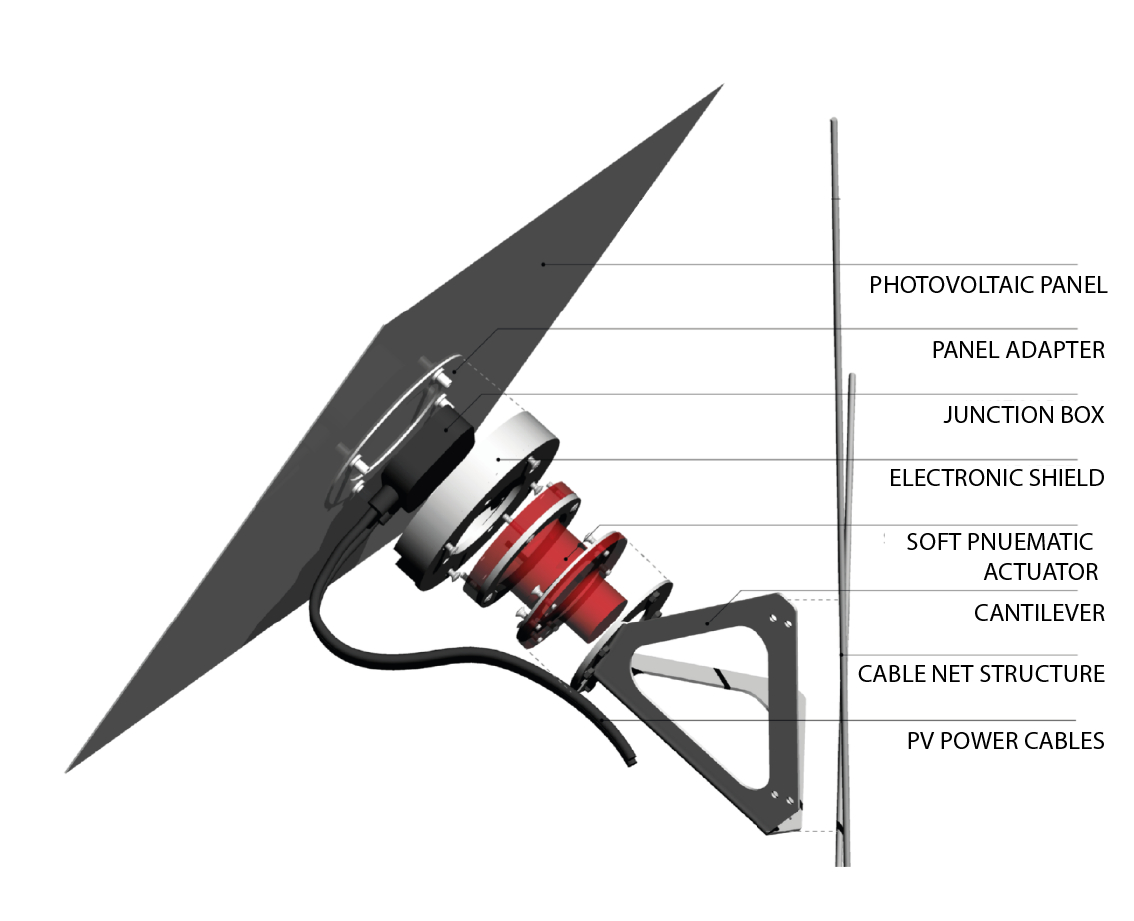
\includegraphics[width=\textwidth, trim= 0cm 0cm 0cm 0cm,clip]{explodedASFV2.png}
\caption{Exploded view of an ASF module mounted on a cable net supporting structure}
\label{fig:explodedView}
\end{center}
\end{figure}

\begin{figure}[ht]
\begin{center}
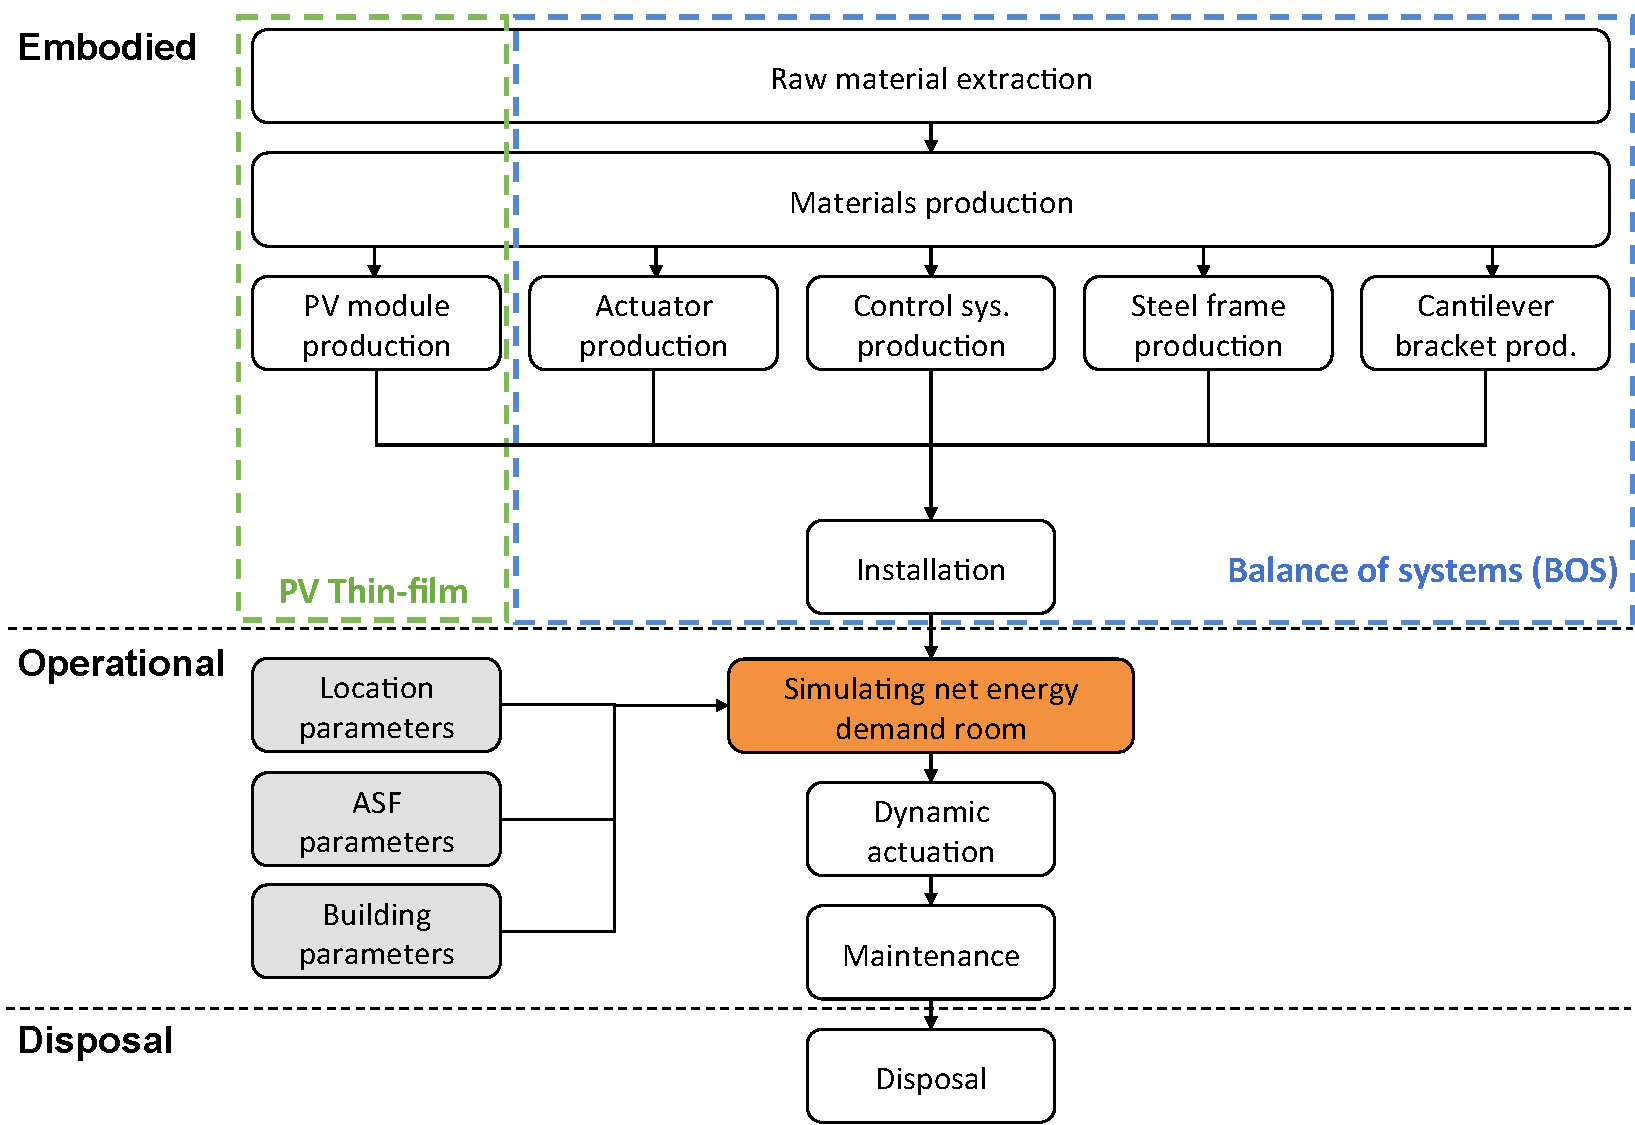
\includegraphics[width=\textwidth, trim= 0cm 0cm 0cm 0cm,clip]{BOS.pdf}
\caption{Breakdown of the ASF into five embodied product components, installation, operation, and disposal}

\label{fig:BOS}
\end{center}
\end{figure}

\begin{description}

\item[PV Panel] \hfill\\
Weight is the primary restriction when selecting a PV panel. Any technology that requires glass encapsulation or a heavy substructure can therefore not be used. The technology also needs to be on the market with high module efficiency. CIGS PV panels were selected as the thin film panel of choice due to its high efficiency, low cost, and ability to be deposited on a polymer or aluminium substrate \cite{chirilua2011highly}. 




\begin{table}[H]
\centering
\begin{tabular}{ll}
\hline
Material description & SMQ \\ \hline
CIGS PV film       	 & 0.569 ${\mathrm{m^2_{PV}/m^2_{facade}}}$\\
Aluminum sheet 	 & 1.593 ${\mathrm{kg/m^2_{facade}}}$\\
Chromium steel panel adapter  & 1.422 ${\mathrm{kg/m^2_{facade}}}$\\
Polyethylene for junction box & 0.036 ${\mathrm{kg/m^2_{facade}}}$\\
Diode, glass for junction box & 0.011 ${\mathrm{kg/m^2_{facade}}}$\\
\hline
\end{tabular}
\caption{Inventory in specific mass quantity (SMQ) of the top five input flows to the PV manufacturing process}
\label{tab:PVinv}
\end{table}

\item[Actuator] \hfill \\
Traditionally photovoltaic actuation is done through the use of servo motors. Servo motors however become a limiting factor for adaptive facades due to their high upfront costs, and instability in heavy winds. Soft robotic actuators on the other hand are cheaper and more resilient to harsh environmental conditions \cite{Svetozarevic2014a}. The soft robotic actuators however are still in development and have an estimated lifetime of five years. They will therefore require three rounds of maintenance during the lifetime of the ASF. For the purpose of this assessment we will run a sensitivity analysis on the use of servo motors and soft robotic actuators. 

\begin{table}[H]
\centering
\begin{tabular}{ll}
\hline
Material description & SMQ \\ \hline
Chromium steel rings	 & 1.0665 ${\mathrm{kg/m^2_{facade}}}$ \\
Electronics, for control, 2-2way valves  & 0.0130  ${\mathrm{kg/m^2_{facade}}}$\\
Silicone chambers & 0.8887 ${\mathrm{kg/m^2_{facade}}}$\\
Polyurethane tubes &0.0933 ${\mathrm{kg/m^2_{facade}}}$\\
Air compressor, screw type, 0.75kW & 1.7281 ${\mathrm{kg/m^2_{facade}}}$\\
\hline
\end{tabular}
\caption{Inventory of four main input flows to the soft robotic actuator manufacturing process }
\label{tab:ActuatorInv}
\end{table}

\item[Cantilever] \hfill \\
The cantilever is a steel connection point between the PV panel and the supporting structure.\\

\begin{table}[H]
\centering
\begin{tabular}{ll}
\hline
Material description & SMQ \\ \hline
Chromium steel bracket	 & 1.4220 ${\mathrm{kg/m^2_{facade}}}$ \\
Chromium steel fixing clamp  & 0.0284 ${\mathrm{kg/m^2_{facade}}}$\\
\hline
\end{tabular}
\caption{Inventory of main input flows to the cantilever manufacturing process }
\label{tab:CantileverInv}
\end{table}

\item[Supporting Structure] \hfill \\
The supporting structure is the connection point between the array of photovoltaic modules and the building itself. Many different designs are possible, however, we will base our analysis of an existing adaptive solar facade \cite{nagy2016adaptive}. This design consists of a steel cable-net that spans a steel supporting frame. The steel frame is then mounted on the building facade.\\

\begin{table}[H]
\centering
\begin{tabular}{ll}
\hline
Material description & SMQ \\ \hline
Chromium steel frame & 6.9928 ${\mathrm{kg/m^2_{facade}}}$ \\
Chromium steel swaged external thread  &0.2897 ${\mathrm{kg/m^2_{facade}}}$\\
Chromium steel wire rope WC  & 0.1593 ${\mathrm{kg/m^2_{facade}}}$\\
\hline
\end{tabular}
\caption{Inventory of the four main input flows to the manufacturing process of the Supporting Structure}
\label{tab:StructureInv}
\end{table}

\item[Control System and Electronics] \hfill \\
The control system is required for the actuation of panels and the regulation of photovoltaic electricity production.\\

\begin{table}[H]
\centering
\begin{tabular}{ll}
\hline
Material description & SMQ \\ \hline
Inverter 1.25kW	 & 0.6090 ${\mathrm{kg/m^2_{facade}}}$ \\
PV cable  &   0.256 ${\mathrm{kg/m^2_{facade}}}$\\
Control Electronics & 0.0516 ${\mathrm{kg/m^2_{facade}}}$\\
\hline
\end{tabular}
\caption{Inventory of the four main input flows to the manufacturing process of the Control System}
\label{tab:ControlInv}
\end{table}

\item[Assembly] \hfill \\
There are many assembly options available. From past experience, an installation of an equivalent ASF required a hydraulic hoist which was in operation for eight hours \cite{jayathissa2015abs}. \\

\begin{table}[H]
\centering
\begin{tabular}{ll}
\hline
Material description & SMQ \\ \hline
Hoist, diesel  ${<}$18.64kW, idling & 0.5267 ${\mathrm{h/m^2_{facade}}}$ \\
\hline
\end{tabular}
\caption{Inventory of main input flows to the Assembly Process}
\label{tab:AssemblyInv}
\end{table}

\end{description}

\subsection{Operational Life Cycle Inventory}
\label{ch:Meth:Opp}

The operational inventory is categorised as 1) energy consumption of an office room 2) electricity consumption through dynamic actuation, and 3) maintenance.

\begin{description}


\item[Building Energy Consumption: ] \hfill\\
An adaptive shading system, when mounted over a glazed facade, has an impact on the energy consumption of the building. More specifically, it has an impact on the heating cooling and lighting loads as described in Section \ref{ch:introduction4}. Previously conducted simulations compared three scenarios: 1) facade with no shading, 2) a facade with a static shading system, optimally angled at 45$^{\circ}$ to the horizontal axis, and 3) an adaptive solar facade \cite{jayathissa2015abs}.\\

The simulation was conducted on a south facing office room. The room, 7.0 meters in length, 4.9 meters wide and 3.1 meters high was modeled using Rhinoceros 3D CAD Package \cite{Rhino}. Grasshopper \cite{grasshopper} was used to model the orientation of each photovoltaic panel. The geometrical input is imported to Energy Plus \cite{energyplus} through the DIVA \cite{DIVA} interface. A single zone thermal analysis was conducted for each possible geometrical configuration of the ASF for each hour of the year. The results were then post processed in MATLAB \cite{MATLAB}.\\

The simulations show a total energy saving of 25\% compared to static panels at 45$^\circ$ and 56\% compared to a case with no facade shading \cite{jayathissa2015abs}. These results are sumarised in Figure \ref{fig:operational}. This data is used to perform our previously described sensitivity analysis which also accounts for HVAC energy savings through adaptive shading. \\




\begin{figure}[H]
\begin{center}

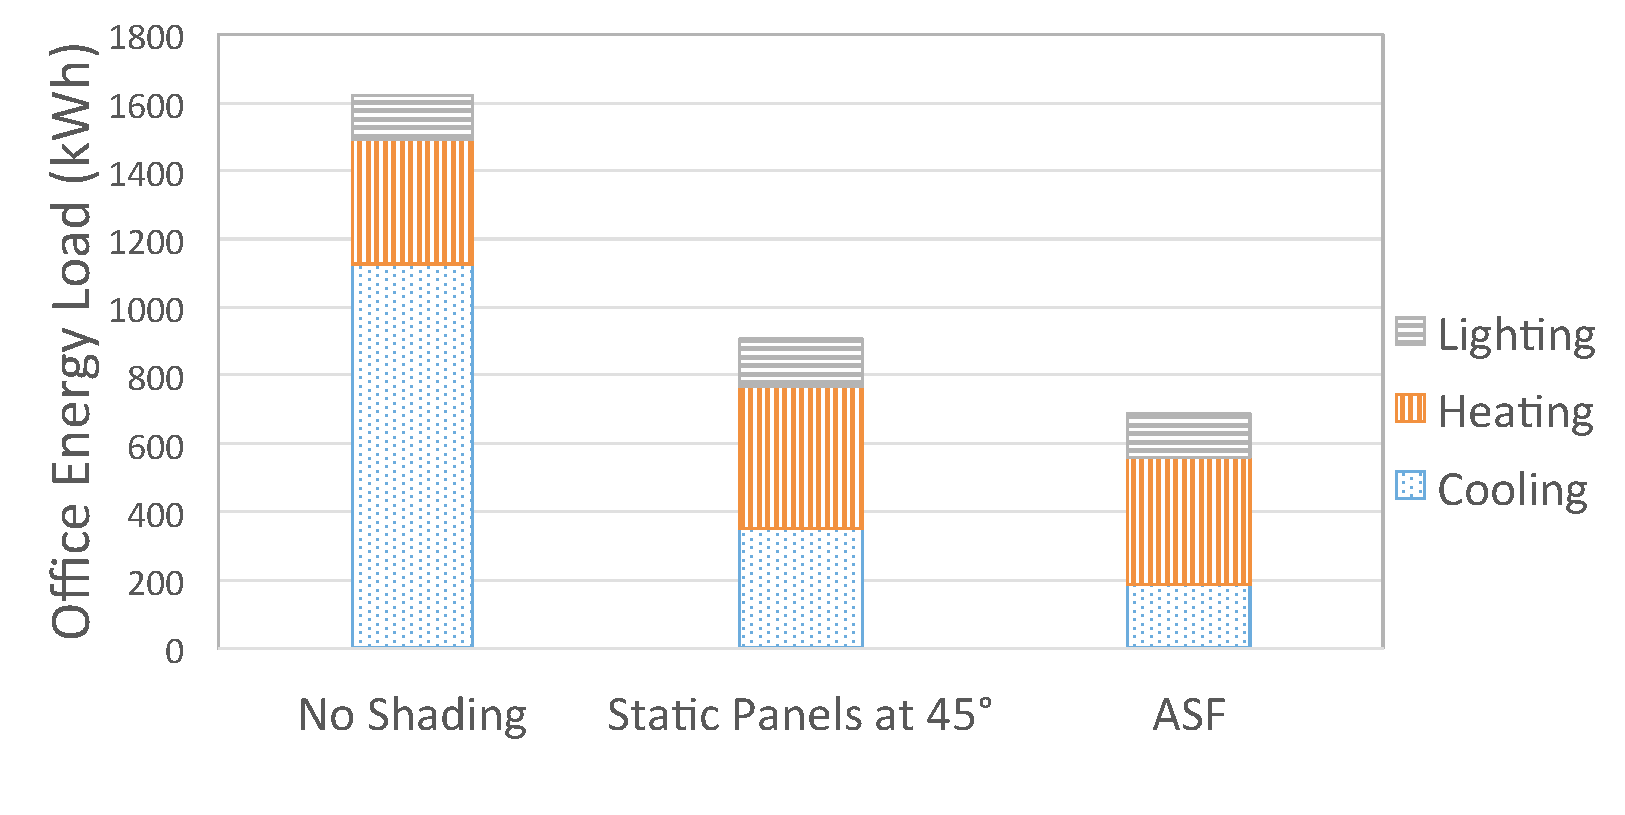
\includegraphics[width=\linewidth, trim= 0cm 0cm 0cm 0cm,clip]{buildingenergy.pdf}
\caption{Breakdown of operational energy consumption for a system in Frankfurt am Main with a) no shading, b) with louvers at 45$^\circ$ and c) with an ASF  -- not including onsite electricity production.}
\label{fig:operational}

\end{center}
\end{figure}


\item[Dynamic Actuation: ] The energy required for actuation is also taken into account. It takes 0.31Wh to fully open a single actuator. Based on the assumption of four full openings and closings per day per actuator, we approximate the combined energy requirement to be 489kWh in its 20 year lifetime. 

\item[Maintenance: ] Soft robotic actuators currently have a lifetime of five years, and therefore will need to be replaced three times during the 20 year lifetime of an ASF. No other maintenance efforts are considered for the assessment of 20 years.

\begin{table}[H]
\centering
\begin{tabular}{ll}
\hline
\textbf{Building Settings}    &                                                \\
Office Envelope               & Roof: Adiabatic                                \\
                              & Floor: Adiabatic                               \\
                              & Walls: Adiabatic                               \\
                              & Window: Double Glazed (e=0.2) 3mm/13mm air \\
Thermal Set Points            & Heating: 22$^{\circ}$C          \\
                              & Cooling: 26$^{\circ}$C          \\
Building System               & Hydronic Heating: COP=4                        \\
                              & Hydronic Cooling: COP=3                        \\
Lighting Control              & Lighting Load: 11.8W/m$^2$                                  \\
                              & Lighting Control: 300 lx Threshhold            \\
Occupancy                     & Office: Weekdays from 8:00-18:00               \\
                              & People set point: 0.1 persons/m$^2$               \\
                              & Infiltration: 0.5 air changes per hour                     \\
                              &                                                \\
\textbf{Location Assumptions} &                                                \\
Weather File                  & Frankfurt am Main, Germany (106370IWEC)               \\
Electricity Mix               & Germany (DE) \cite{itten2012life}                   \\
Average Solar Radiation               & 855kWh/m$^2$/year                              \\
                              &                                                \\
\textbf{Maintenance}          &                                                \\
Actuator Changes              & Every 5 years                                  \\
                              &                                                \\
\textbf{ASF Assumptions}         &                                                \\
Full openings and closings  & 4 per day                                      \\
\hline
\end{tabular}
\caption{Summary of main assumptions for the calculation of operational emissions}
\label{tab:AssumptionsOpp4}
\end{table}


\end{description}



\subsection{Sensitivity Analysis}
\label{ch:meth:sens}

In order to evaluate the impact of varying parameters on the LCA, we performed a sensitivity analysis on the following assumptions
\begin{itemize}
\item When an ASF is built over a glazed building surface, thus including the effects of adaptive shading on the building energy consumption.
\item The location of the ASF including the effects of the GWP of the local electricity mix. Assessments will also be run in Madrid and Geneva.
\item A static version of the ASF, where panels are optimally orientated at 45$^{\circ}$ to the horizontal (altitude) axis.
\item The type of actuation system (servo motors compared to soft robotic actuators).
\item The complexity of the control system. The ASF can be built where each panel is independently actuated, or a case where it is actuated in rows. When the panels are actuated independently more valves and control electronics are required.

\end{itemize}
